\documentclass[../TinyBot.tex]{subfiles}
% \graphicspath{{resources/}}
\begin{document}

\section{Wiring} \label{wiring}
If you just want to see the wiring schematic, see Figure \ref{fig:schematic-hbridge-battery}.
Continue reading for an explanation of the L293D H-Bridge and of the circuit. 

\bigskip

Before starting construction on any project, it is always a good idea to wire up the circuit
on a flat breadboard and Arduino, as it is far easier to build the circuit on its own before
putting together all the parts. \\

\begin{center}
    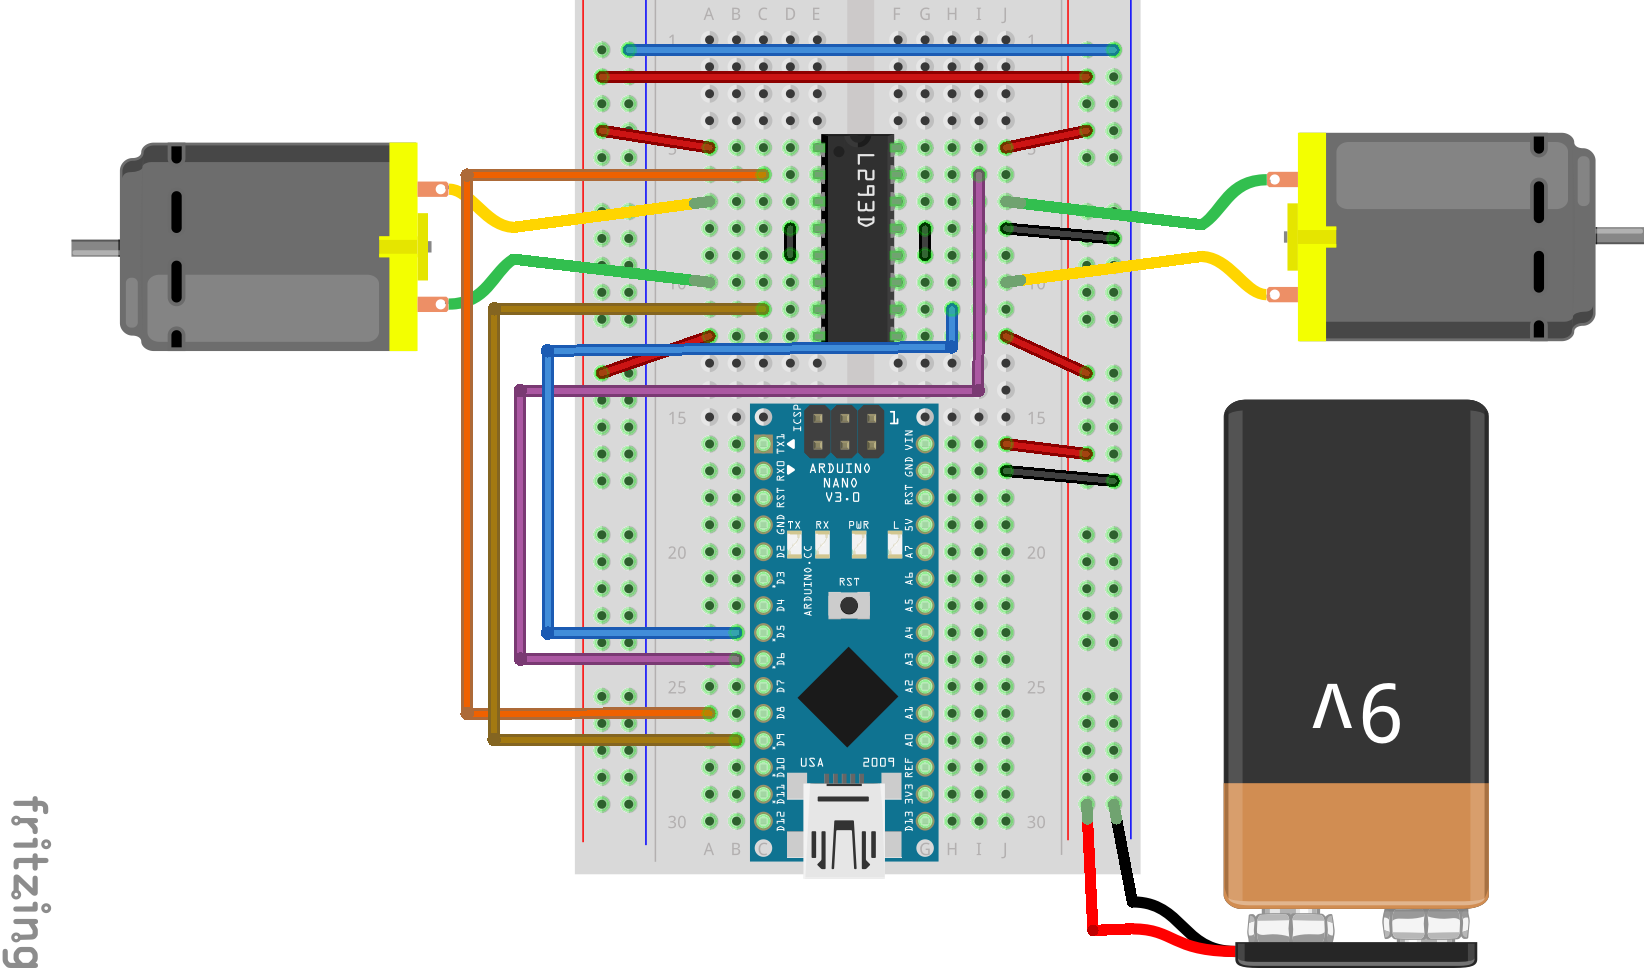
\includegraphics[width=\textwidth]{resources/H-bridge-nano_bb.png}
    \captionof{figure}{Wiring Schematic for H-Bridge}
    \label{fig:schematic-hbridge-battery}
\end{center}

Make sure to check which wire is the positive wire on the motor you have, it should be written
on the back plate of the motor. Plugging the motor in backwards will not break anything,
the motor will just spin backwards. Swapping the motor direction can be done by swapping
the green and yellow wires attached to the motor. \\
% It is mainly important to ensure that the motors spin in the same direction. 

\newpage

If you don't have a battery, the circuit is mostly the same, though with some differences
with how power is supplied to the circuit. Instead of powering the Arduino and circuit
with the 9V battery you power the Arduino through USB and the circuit from the 5V output pin.
See figure \ref{fig:schematic-hbridge-nobattery} below for a wiring diagram without the battery.

\begin{center}
    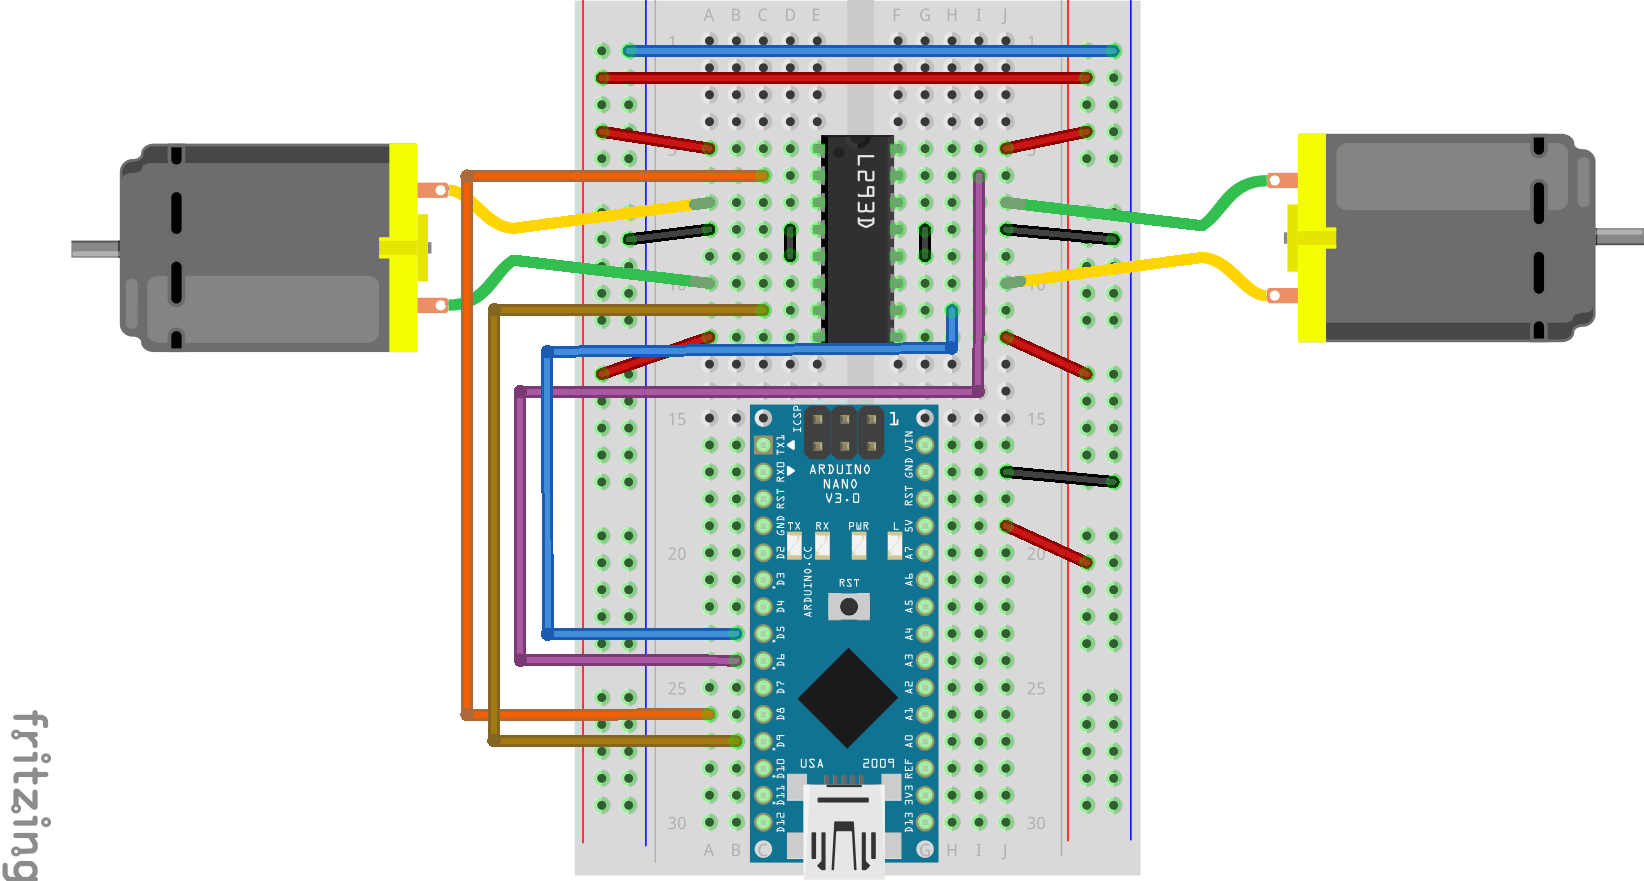
\includegraphics[width=\textwidth]{resources/H-bridge-nano-without-battery_bb.png}
    \captionof{figure}{Wiring Schematic for H-Bridge}
    \label{fig:schematic-hbridge-nobattery}
\end{center}


\end{document}